\fig{fv:c4:arrival}{相同初值的衰减可以在有限时刻终止，也可以渐近趋零}{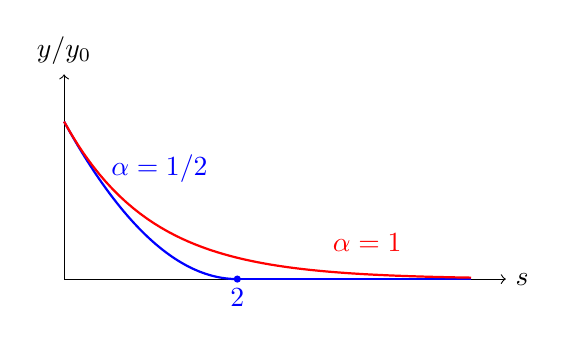
\begin{tikzpicture}[x=1.1cm,y=2cm]
\draw[->](0,0)--(5.1,0)node[right]{$s$};\draw[->](0,0)--(0,1.3)node[above]{$y/y_0$};
\draw[blue,thick,domain=0:2,samples=60]plot(\x,{(1-\x/2)^2});\draw[blue,thick](2,0)--(4.7,0);
\draw[red,thick,domain=0:4.7,samples=60]plot(\x,{exp(-\x)});
\fill[blue](2,0)circle(1.3pt)node[below]{$2$};\node[red]at(3.5,.23){$\alpha=1$};\node[blue]at(1.1,.7){$\alpha=1/2$};
\end{tikzpicture}}
图\ref{fv:c4:arrival}用 $s=ky_0^{\alpha-1}t$消去单位。$\alpha=1/2$时 $y/y_0=(1-s/2)^2$只在 $0\le s\le2$表示下降支路；此后按非负模型接到 $y=0$。若把平方式直接延长到 $s>2$，它反而增大，已经不满足原来的负导数方程。$\alpha=1$的指数曲线在任意有限 $s$仍为正。图形的触轴方式因此对应不同的到达时间，必须与方程和允许状态一起判断。
